\chapter{Theoretical Framework}


\section{Gravitational waves theory}
After considering, in 1905, the problem of the apparently \textit{instantaneous} propagation of light, with the theory of Special Relativity, in 1916 Albert Einstein considered the problem of the apparently \textit{instantaneous} propagation of gravity through \textit{long distances}, in his theory of General Relativity.
Einstein showed that long-distance interaction arises from the deformation of space time caused by massive objects.
Hence, in the "static case", the deviated motion apparently caused by the interaction between two distant masses really is, in fact, a manifestation of space time curvature nearby, generated by the presence of the two objects.
The "static case" just depicted, though, treats the curvature as if it had always been there, and doesn't take into account of any variation in the masses, positions or velocities of the two objects, that would induce an evolution to the curvature itself.
In truth, after a change in the mass-energy distribution, the corresponding curvature variation requires its time to reach far distances, and a fascinating prediction of General Relativity is that it propagates in the form of a wave, that travels at the speed of light.
For the treatment that follows, I have primarily relied on \cite{ferrari2020general}, particularly Chapters 12, 13, and 14.
I will not go into the full mathematical derivations here, but they are presented in detail in the book.

\subsection{Gravitational Waves as Perturbations}
The typical approach to the study of gravitational waves is to derive them as small perturbations of the background from the Einstein's equations: 
\begin{equation}
    G_{\mu\nu} = R_{\mu\nu} - \frac{1}{2}g_{\mu\nu}R,
\end{equation}
which can be conveniently written as 
\begin{equation}
    R_{\mu\nu}=\frac{8\pi G}{c^4}\left(T_{\mu\nu} - \frac{1}{2}g_{\mu\nu}T\right),
    \label{eq: Einstein equations rewritten}
\end{equation}
where $G_{\mu\nu}$ is the Einstein tensor, $R_{\mu\nu}$ is the Ricci tensor, $R$ is the Ricci scalar, $g_{\mu\nu}$ is the metric of space time, and $T_{\mu\nu}$ is the stress-energy tensor.
As a background solution we can consider the flat space time described by the metric $\eta_{\mu\nu}$, to which the perturbation term appears as a fluctuation in the metric $|h_{\mu\nu}|\ll|\eta_{\mu\nu}|$, known as \textit{weak field} approximation. Thus, the perturbed space time can be written as:
\[
    g_{\mu\nu} = \eta_{\mu\nu} + h_{\mu\nu}, \hspace{5mm}  |h_{\mu\nu}|\ll|\eta_{\mu\nu}|.
\] 
With this metric, the equations \ref{eq: Einstein equations rewritten} becomes
\[
    \{\square_F h_{\mu\nu} - \left[\frac{\partial^2}{\partial x^\lambda\partial x^\mu}h^\lambda_\nu + \frac{\partial^2}{\partial x^\lambda\partial x^\nu}h^\lambda_\mu + \frac{\partial^2}{\partial x^\nu\partial x^\mu}h^\lambda_\lambda\right]\} = -\frac{16\pi G}{c^4}\left(T_{\mu\nu} - \frac{1}{2}\eta_{\mu\nu}T\right).
\]
Now, by requiring that the \textit{weak-field} approximation remains satisfied for infinitesimal diffeomorphisms, and by choosing a coordinate system in which the \textit{harmonic gauge condition}\footnote{It is an arbitrary coordinate condition which makes it possible to solve the Einstein field equations. It can be found by requiring that the linearized Einstein equations satisfy the D'Alambert equation.}, defined as 
\begin{equation}
    \Gamma^\lambda = g^{\mu\nu}\Gamma^\lambda_{\mu\nu} = 0,
    \label{eq: Harmonic gauge definition}
\end{equation}
where $\Gamma^\lambda_{\mu\nu}$ are the \textit{affine connections}, is satisfied, we can find that, up to first order in $h_{\mu\nu}$, the harmonic gauge condition is equivalent to 
\begin{equation}
    \frac{\partial}{\partial x^\mu}h^\mu_\rho = \frac{1}{2}\frac
    {\partial}{\partial x^\rho}h, \hspace{5mm} h=\eta^{\mu\nu}h_{\mu\nu}\equiv h^\nu_\nu.
\end{equation}
After defining the \textit{trace-reversed}\footnote{The name comes by noting that $\bar{h}=\eta^{\mu\nu}\bar{h}_{\mu\nu} = -h$.} tensor as
\begin{equation*}
    \bar{h}_{\mu\nu} \equiv h_{\nu\mu} - \frac{1}{2}\eta_{\mu\nu}h,
\end{equation*}
we can finally write the linearized Einstein equations as
\begin{equation}
    \left\{
        \begin{aligned}
            \square\bar{h}_{\mu\nu} &= -\frac{16\pi G}{c^4} T_{\mu\nu}, 
            \notag\\
            \partial^\mu \bar{h}_{\mu\nu} &= 0.
        \end{aligned}
    \right.
    \label{eq: Einstein equations as wave equations}
\end{equation}
This form, and its twin with $T_{\mu\nu}=0$, where the first equation becomes the D'Alambert equation, are relevant because they show that \textit{a perturbation of a flat space time propagates as a wave travelling at the speed of light}.
As in Electrodynamics, the solution of~\eqref{eq: Einstein equations as wave equations} can be written in terms of \textit{retarded potentials}:
\begin{equation}
    \bar{h}_{\mu\nu}(t,\mathbf{x}) = \frac{4G}{c^4}\int_V \frac{T_{\mu\nu}(t - \frac{|\mathbf{x} - \mathbf{x}'|}{c}, \mathbf{x}')}{|\mathbf{x} - \mathbf{x}'|}d^3x',
    \label{eq: solutions with retarded potentials}
\end{equation}
where V is the three dimensional source volume, $\mathbf{x}'$ is the distance of an element of the emitting source from the origin of a frame centered in the same point of the source, $\mathbf{x}$ is the distance between source and observer.
It can be proved that the solutions in~\eqref{eq: solutions with retarded potentials} automatically satisfy the harmonic gauge condition.

\subsubsection{Harmonic gauge}
It is important to notice that if the \textit{harmonic gauge} condition is not satisfied in a reference frame, a new frame in which it is can always be found, by making an infinitesimal coordinate transformation
\begin{equation}
    x^{\lambda'} = x^\lambda + \epsilon^\lambda,
    \label{eq: infinitesimal coordinate transformation}
\end{equation}
provded that $\epsilon^\lambda$ satisfies the following equation:
\[
    \square_F\epsilon_\rho = \frac{\partial h^\beta_\rho}{\partial x^\beta} - \frac{1}{2} \frac{\partial h}{\partial x^\rho} = 0\hspace{1mm}.
\]
This is an inhomogeneous wave equation that can be solved to find the components $\epsilon_\alpha$, which identify the coordinate system in which the harmonic gauge condition is satisfied.
Notice though, that the harmonic condition in \eqref{eq: Harmonic gauge definition} does not determine the gauge uniquely, but instead leaves some more gauge freedom to be used.

\subsection{The physical wave}
As we have seen, perturbations of flat space-time satisfy a wave equation and a harmonic gauge condition, as in \eqref{eq: Einstein equations as wave equations}.
The general solutions of these wave equation is a linear superposition of monochromatic plane waves, with a polarization tensor (or wave amplitude) $A_{\mu\nu}$ and a wave four-vector $\vec{k}$, such as
\[
    \square_F \bar{h}{\mu\nu} = -A_{\mu\nu}\eta^{\alpha\beta} k_\alpha k_\beta e^{ik_\gamma x^\gamma} = 0.
\]
Thus, neglecting the trivial solution $A_{\mu\nu} = 0$, gives 
\[
    \eta^{\alpha\beta} k_\alpha k_\beta = 0,
\]
which means that $\vec{k}$ is a null vector.
If we also consider the harmonic gauge, we find a condition that imposes the orthogonality  of the wave four-vector to the polarization tensor,
\[
    k_\mu A^\mu_\nu = 0.
\]
The \textit{wavefronts}, i.e. the spatial surfaces where $\bar{h}_{\mu\nu}= const.$ are the planes where $k_ix^i=const.$
Conventionally, $k^0$ is referred to as $\frac{\omega}{c}$, where $\omega$ is the frequency, thus
\[
    \vec{k}_0 = \left(\frac{\omega}{c},\mathbf{k}\right),
\]
where $\mathbf{k}$ is the wave three-vector orthogonal to the wavefront, and is related to the \textit{wavelenght} by $|\mathbf{k}| = 2\pi/\lambda$.
Notice that, since the wave four-vector $\vec{k}$ is a null vector, it follows that
\[
    -(k^0)^2 + |\mathbf{k}| = 0 \to \omega = ck_0 = c|\mathbf{k}|,
\]
which gives the dispersion relation for a wave moving at the speed of light.


\subsubsection{The TT gauge}
In a one dimension case, the wave equation can be written as
\[
    \left( -\frac{1}{c^2} \frac{\partial^2}{\partial t^2}  + \frac{\partial^2}{\partial x^2}\right)\bar{h}^\mu_\nu = 0,
\]
which generally has, as solution, an arbitrary function of $t\pm \frac{x}{c}$.
If we consider, for example, a progressive wave $\bar{h}^\mu_\nu [f(t,x)]$, where $f(t,x) = t- \frac{x}{c}$, and apply the harmonic gauge condition, focusing only in the time-dependent part of the solution, we find the \textit{first four} conditions:
\begin{equation}
    \bar{h}^t_t = \bar{h}^x_t, \hspace{5mm} \bar{h}^t_x = \bar{h}^x_x, \hspace{5mm} \bar{h}^t_y = \bar{h}^x_y, \hspace{5mm} \bar{h}^t_z = \bar{h}^x_z.
    \label{eq: first four conditions}
\end{equation}
As we have already discussed, there still is the freedom of making an infinitesimal coordinate change, and by requiring that the harmonic gauge remains satisfied in the new coordinates generates \textit{four more conditions}:
\begin{equation}
    \bar{h}^t_x = \bar{h}^t_y = \bar{h}^t_z = \bar{h}^y_y + \bar{h}^z_z = 0,
    \label{eq: second four conditions}
\end{equation}
and with the~\eqref{eq: first four conditions} follows
\[
     \bar{h}^x_x = \bar{h}^x_y = \bar{h}^x_z = \bar{h}^t_t = 0.
\]
The only non zero components are $\bar{h}^z_y$ and $\bar{h}^y_y - \bar{h}^z_z$, which cannot be set to zero because now we have completely used all the gauge freedom.
It can be shown that, from all the above conditions, it follows that $\bar{h} \equiv h$, i.e. in this gauge the wave results to be \textit{traceless}.
Thus, a plane gravitational wave propagating along the $x$-axis is characterized by only two non-zero functions $h_{zy}$ and $h_{yy}=-h_{zz}$:
\begin{equation}
    h^{TT}_{\mu\nu} =  
    \begin{pmatrix}
0 & 0 & 0 & 0 \\
0 & 0 & 0 & 0 \\
0 & 0 & h_{yy} & h_{yz} \\
0 & 0 & h_{yz} & -h_{yy}
\end{pmatrix}.
    \label{eq: h as a matrix in x case}
\end{equation}
In conclusion, the gravitational wave only has \textbf{two physical degrees of freedom} which correspond to two polarization states.
This gauge is called \textbf{TT gauge} because of the \textit{transverse traceless} nature: $h_{\mu\nu}$ is traceless, thus $h=0$, and transverse, since the components of $h_{\mu\nu}$ along the direction of propagation are null (in this case $h_{\mu_x}=0$).

\subsection{Motion and geodesics}
Free test particles in General Relativity move along geodesic, which means that, in terms of a world line $x^\mu(\tau)$ parametrized by proper time $\tau$, they satisfy the \textit{geodesic equation}:
\begin{equation}
    \frac{d^2x^\alpha}{d\tau^2} + \Gamma^\alpha_{\mu\nu} \frac{dx^\mu}{d\tau}\frac{dx^\nu}{d\tau} \equiv \frac{du^\alpha}{d\tau} + \Gamma^\alpha_{\mu\nu}u^\mu u^\nu = 0,
    \label{eq: geodesic equation of free particle}
\end{equation}
where $u^\alpha = \frac{dx^\alpha}{d\tau}$ is the particle velocity.
By imposing the rest condition, $u^\alpha = (1,0,0,0)$, to the~\eqref{eq: geodesic equation of free particle} and considering the TT gauge component prescriptions for $h_{\mu\nu}$, we find that a particle initially at rest is not accelerated by the passage of a wave, but remains at a fixed coordinate position: the motion of a single particle is not affected by the gravitational waves.

\subsubsection{The geodesic deviation}
If we consider, instead, the relative motion of close particles, the situation is different.
This relative motion is governed by the \textit{geodesic deviation}, which quantifies how two very close geodesics deviate from one another.
Although, as we have seen, the coordinates of the two particles (and thus their difference) do not change when a gravitational wave passes, this does not hold true for their \textit{proper distance} o
\[
    \Delta l = \int ds \not = const.
\]
This apparent contradiction arises from the fact that the coordinate difference is not a \textit{tensorial} quantity, and therefore is not suited to describe properly a physical process.
This is the reason we consider the geodesic deviation, which provides a tensorial formulation of the relative acceleration between the two particles: 
\begin{equation}
    \frac{D^2\delta x^\alpha}{d\tau^2} \equiv (\Delta_{\vec{t}}(\Delta_{\vec{t}}\vec{\delta x}))^\alpha = R^\alpha_{\beta\mu\nu}t^\beta t^\mu \delta x^\nu,
    \label{eq: geodesic deviation}
\end{equation}
where 
\begin{equation}
    R_{\alpha k \lambda \mu} = \frac{1}{2}( g_{\alpha\mu,\lambda k}  + g_{k\lambda,\mu \alpha }  - g_{\alpha\lambda,\mu k }  - g_{k\mu,\lambda \alpha })
    \label{eq: Riemann tensor def}
\end{equation}
is the Riemann curvature tensor, $\vec{t}$ is the tangent vector to one of the geodesic, and $\vec{\delta x}$ is a deviation vector between the two geodesics.
it is important to note that in the presence of a gravitational wave the Riemann tensor is never zero in any reference frame, and consequently neither is the geodesic deviation. 
In contrast, the quantity $\frac{d^2\delta x^i}{d\tau^2}$ (which is not a tensorial quantity) vanishes in the TT frame.

Knowing this, to analyze this effect in more detail we can choose to integrate the~\eqref{eq: geodesic deviation} in a \textit{Locally Inertial Frame}, LIF \{$\xi^\alpha$\}, centered on one of the two particles, where the metric can be approximated close to the origin as Minkowski up to quadratic, negligible, corrections:
\[
    ds^2 = \eta_{\alpha\beta} d\xi^\alpha d\xi^\beta + O(|\xi|^2).
\]
In this frame, the Riemann tensor in~\eqref{eq: Riemann tensor def}, which depends on second derivatives of the metric perturbation $h_{\mu\nu}$ (with $g_{\mu\nu} = \eta_{\mu\nu} + h_{\mu\nu}$), is not only covariant, but actually \textit{invariant} under infinitesimal coordinate transformations from a generic LIF to the TT frame. 
This is especially useful because in the TT frame $h^{TT}_{\mu\nu}$ takes a particularly simple form, as we have seen in the~\eqref{eq: h as a matrix in x case} example, simplifying also the expression for $R^{TT}_{\alpha k \lambda \mu}$. 
Assuming that the wave travels along the $\xi^1$ direction, the solutions for the geodesic deviation equation for two close particles are the non zero components of 
\begin{equation}
    \delta\xi^j = \delta\xi_0^j + \frac{1}{2}\eta^{ji} h^{TT}_{ik} \delta\xi_0^k,
    \label{eq: solution of geodesic deviation}
\end{equation}
where $\delta\xi_0^j$ represent the initial, constant separaion between the particles. 
As previously discussed, the non-zero components of the strain tensor $h_{ik}^{TT}$ correspond to two possible polarizations of the gravitational wave. 
Their distinct effects on a ring of close particles are viually represented in \textbf{Figure~\ref{fig:gw_polarizations}}.
\begin{figure}[h]
    \centering
    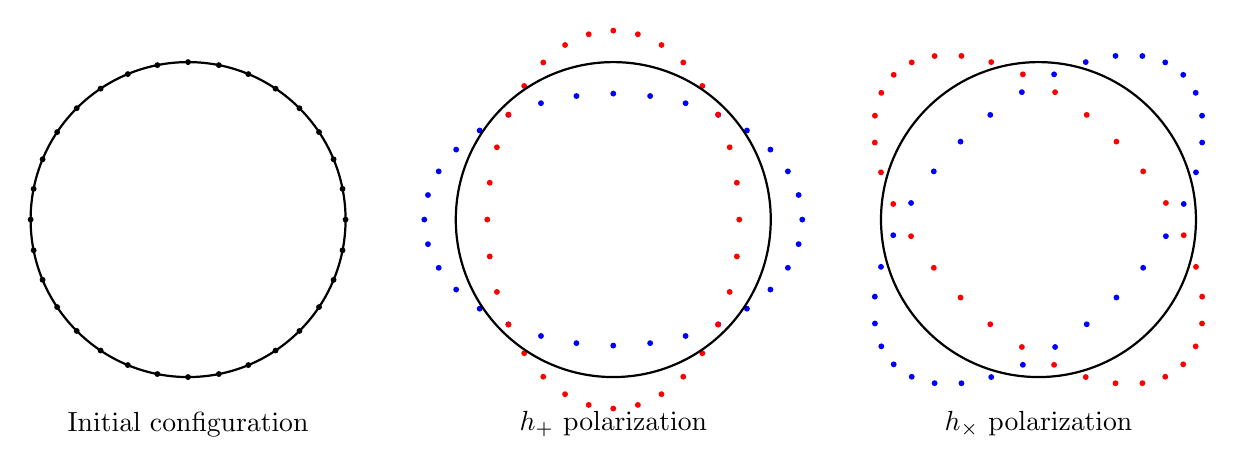
\begin{tikzpicture}[scale=2]

    % Configurazione iniziale (cerchio)
    \foreach \angle in {0,11.25,...,348.75}{
        \node[circle,fill=black,inner sep=0.75pt] at (\angle:1) {};
    }
    \draw[thick] (0,0) circle(1);
    \node at (0,-1.3) {Initial configuration};

    % Polarizzazione +
    \begin{scope}[xshift=2.7cm]
        % Fase 1: ellisse orizzontale
        \foreach \angle in {0,11.25,...,348.75}{
            \pgfmathsetmacro{\x}{cos(\angle)}
            \pgfmathsetmacro{\y}{sin(\angle)}
            \node[circle,fill=black,inner sep=0.75pt,blue]
                at ({1.2*\x},{0.8*\y}) {};
        }
        % Fase 2: ellisse verticale
        \foreach \angle in {0,11.25,...,348.75}{
            \pgfmathsetmacro{\x}{cos(\angle)}
            \pgfmathsetmacro{\y}{sin(\angle)}
            \node[circle,fill=black,inner sep=0.75pt,red]
                at ({0.8*\x},{1.2*\y}) {};
        }
        % Cerchio di riferimento
        \draw[thick] (0,0) circle(1);
        \node at (0,-1.3) {${h}_{+}$ polarization};
    \end{scope}

    % Polarizzazione ×
    \begin{scope}[xshift=5.4cm]
        % Fase 1: shear a +45°
        \foreach \angle in {0,11.25,...,348.75}{
            \pgfmathsetmacro{\x}{cos(\angle)}
            \pgfmathsetmacro{\y}{sin(\angle)}
            \pgfmathsetmacro{\xp}{\x + 0.3*\y}
            \pgfmathsetmacro{\yp}{\y + 0.3*\x}
            \node[circle,fill=black,inner sep=0.75pt,blue] at (\xp,\yp) {};
        }
        % Fase 2: shear a -45°
        \foreach \angle in {0,11.25,...,348.75}{
            \pgfmathsetmacro{\x}{cos(\angle)}
            \pgfmathsetmacro{\y}{sin(\angle)}
            \pgfmathsetmacro{\xp}{\x - 0.3*\y}
            \pgfmathsetmacro{\yp}{\y - 0.3*\x}
            \node[circle,fill=black,inner sep=0.75pt,red] at (\xp,\yp) {};
        }
        % Cerchio di riferimento
        \draw[thick] (0,0) circle(1);
        \node at (0,-1.3) {${h}_{\times}$ polarization};
    \end{scope}

    \end{tikzpicture}
    \caption{Effect of the two gravitational wave polarizations on a ring of free-falling particles, caused by a wave moving in the direction perpendicular to the page: blue and red dots represent two opposite phases of the wave.}
    \label{fig:gw_polarizations}
\end{figure}

\subsection{The quadrupole approximation}
Now that we have discussed the effects of the passage of a gravitational wave on the relative motion of close particles, we can focus on another important ptoblem: \textit{how such waves are generated}.
Gravitational radiation is a consequence of variations in the spacetime curvature, and it generates from time-dependent distributions of mass and momentum.
But not every motion of matter can produce gravitational wave signal, as we will see: conservation laws of general relativity, impose strict constraints on the possible multipole moment that can contribute to the tensorial metric perturbations.


\subsubsection{The weak-field, slow-motion approximation}
We already introduced previously the weak-field limit, which allows us to write the metric as a perturbed Minkowski $g_{\mu\nu}=\eta_{\mu\nu} + h_{\mu\nu}$, with $|h_{\mu\nu}|\ll 1$, and we found the solutions as in~\eqref{eq: Einstein equations as wave equations}.
Until now, we have only solved these equations with a null stress-energy tensor.
If we assume that the region, of size $\epsilon$, where the source of the signal is confined, is much smaller than the wavelenght of the emitted gravitational radiation, $\lambda_{GW} = \frac{2\pi c}{\omega}$, we find the following condition:
\begin{equation}
    \frac{2\pi c}{\omega}\gg \epsilon \to \epsilon\omega \ll c \to v_{typical} \ll c.
    \label{eq: slow motion approximation}
\end{equation}
The typical velocities of the system are much smaller than the speed of light: this is the so called \textit{slow motion approximation}.
If we now use the solution found using the retarded potentials in~\eqref{eq: solutions with retarded potentials}, by making use of the Fourier transforms it can be found that the gravitational wave signal emitted by the source, to leading order in the weak-field, slow-motion approximation is
\begin{equation}
    \bar{h}_{\mu\nu}(t,r) = \frac{4G}{rc^4}\int_V T_{\mu\nu}(t-\frac{r}{c}, \mathbf{x}')d^3x.
    \label{eq: weak-field slow-motion solutions}
\end{equation}

\subsubsection{The quadrupole formula}
The integral in~\eqref{eq: weak-field slow-motion solutions} can be simplified with some expedients. 
First of all, by making use of the conservation law that applies to the stress-energy tensor
\[
    \frac{\partial T^{\mu\nu}}{\partial x^\nu}=0, \hspace{4mm} \to \hspace{4mm} \frac{1}{c}\frac{\partial T^{\mu 0}}{\partial t} = - \frac{\partial T^{\mu\nu}}{\partial x^k}, \hspace{4mm} \mu=0,\dots,3,\hspace{2mm} k=1,2,3,
\]
a smart use of the Gauss' theorem (reminding that the stress-energy tensor is null on the source's surface), it can be found that 
\[
    \bar{h}^{\mu\nu}=0.
\]
Secondly, we can use the \textbf{tensor-virial theorem}
\begin{equation}
    \frac{1}{c^2}\frac{\partial^2}{\partial t^2}\int_V T^{00}x^kx^nd^3x = 2\int_V T^{kn}d^3x, \hspace{3mm} k,n=1,2,3,
    \label{eq: tensor-virial theorem}
\end{equation}
in the definition of the \textbf{quadrupole moment tensor}
\begin{equation}
    q^{kn}(t) = \frac{1}{c^2}\int_VT^{00}(t,\mathbf{x})x^kx^nd^3x,
    \label{eq: quadrupole moment tensor}
\end{equation}
we finally find that~\eqref{eq: weak-field slow-motion solutions} can be re-written as
\begin{align}
   &\bar{h}^{\mu 0} =0,\notag\\
   &\bar{h}^{ik}(t,r) = \frac{2G}{c^4r}\frac{d^2}{dt^2}q^{ik}(t-\frac{r}{c}),
    \label{eq: quadrupole formula}
\end{align}
known as the \textbf{quadrupole formula}.
This formulation describes the gravitational wave signal emitted by a gravitating system that evolves in time, whatever the mass-energy distribution looks like, as long as $\ddot{q}^{ik}\not = 0$.
Note that in this approximation, the only component of the stress-energy tensor that generates the metric perturbation is $T^{00}$, and that the $c^{-4}$ rendes the characteristic strain extremely small:
\[
    \frac{G}{c^4}\sim 10^{-49}\frac{s^2}{g\hspace{1mm}cm}.
\]

\subsubsection{Transform to the TT gauge}
The solution in~\eqref{eq: quadrupole formula} represents a spherical wave far from the source, which locally looks like a plane wave.
It can also be expressed, after an infinitesimal coordinate trasformation that preserves the harmonic gauge.
This projection in the TT gauge is performed by defining symmetric and transverse \textit{projector operators} as
\[
    P_{jk}\equiv \delta_{jk} - n_jn_k,
\]
to than define the \textbf{transverse-traceless projector} 
\begin{equation}
    P_{jkmn}\equiv P_{jm}P_{kn}-\frac{1}{2}P_{jk}P_{mn},
    \label{eq: transverse-traceless projector}
\end{equation}
which "extracts" the transverse-traceless part of a rank two tensor on the three-dimensional Euclidean space.
This way we can, for example, define
\[
    h_{jk}^{TT} = P_{jkmn}\bar{h}_{mn},
\]
that, if applied to the~\eqref{eq: quadrupole formula}, gives
\begin{align}
   &\bar{h}^{TT}_{\mu 0} =0,\notag\\
   &\bar{h}^{TT}_{ik}(t,r) = \frac{2G}{c^4r}\frac{d^2}{dt^2}Q^{TT}_{ik}(t-\frac{r}{c}),
   \label{eq: TT part of quadrupole moment}
\end{align}
where $Q_{jk}^{TT} = P_{jkmn}q_{mn}$ is the \textbf{transverse-traceless part of the quadrupole moment}.
As we will see, to compute the "luminosity" of a gravitational wave source, it is useful to define the \textbf{reduced quadrupole moment}
\begin{equation}
    Q_{jk} \equiv q_{jk} - \frac{1}{3}\delta_{jk}q_m^m, 
    \label{eq: reduced quadrupole moment}
\end{equation}
which is traceless by definition.

\subsubsection{Gravitational waves from a binary system}
As an example, we can consider a binary system where two masses $m_1$ and $m_2$ are in a circular orbit around the common center of mass.
The typical parameters are the total mass
\[
    M\equiv m_1+m_2,
\]
the \textit{reduced mass}
\[
    \mu\equiv \frac{m_1m_2}{M},
\]
and, by placing the origin of the coordinate frame in the center of mass, 
\[
    l_0 = r_1+r_2, \hspace{3mm} r_1=\frac{m_2}{M}l_0, \hspace{3mm} r_2=\frac{m_1}{M}l_0, \hspace{3mm} \omega_K=\sqrt{ \frac{GM}{l_0^3}}.
\]
Now, after defining the coordinates of the masses $(x_1,y_1)$ and $(x_2,y_2)$ in an orbital plane, orthogonal to the $z$-axis, as functions of all the above parameters, it becomes possible to compute the 00-component of the stress-energy tensor as
\[
T^{00}=c^2\sum^2_{n=1}m_n\delta(x-x_n)\delta(y-y_n)\delta(z),
\]
and thus all the non-vanishing components of $q_{jk}$.
From this we can find $Q_{jk}$, $Q_{jk}^{TT}$, and finally
\begin{equation}
    h_{ij}^{TT}(t,r) = -\frac{A}{r}A_{ij}^{TT}(t-\frac{r}{c}),
    \label{eq: binary system general strain solution}
\end{equation}
where\footnote{Note that this shows that a \textit{binary system in circular orbits emits waves at twice the orbital frewuency}} 
\begin{align}
    & A=\frac{4\mu MG^2}{l_0c^4}, \notag\\
    & A_{ij}^{TT}(t-\frac{r}{c}) = P_{ijkl}A_{kl}(t-\frac{r}{c}),\notag\\ 
    \vspace{2mm}
    &    A_{kl}(t) =  
    \begin{pmatrix}
        \cos{2\omega_Kt} & \sin{2\omega_Kt} & 0 \\
     \sin{2\omega_Kt} &  -\cos{2\omega_Kt}& 0 \\
     0 & 0 & 0 \\
    \end{pmatrix}.
    \label{eq: A definition}
\end{align}
Using typical values, such as the PSR 1913+16 assuming it had a circular orbit, by defining 
\[
    h_0=\frac{A}{r},
\]
and using~\eqref{eq: A definition}, we find  
\begin{equation}
    h_0\sim 5\times10^{-23}, 
    \label{eq: typical strain amplitude value}
\end{equation}
as an estimate of a typical gravitational wave signal amplitude generated by a binary system.

\subsection{Energy carried by a gravitational wave}
The stress-energy tensor conservation laws that we know in Special relativity
\[
    T^{\mu\nu}_{,\nu}=0,
\]
unfortunately do not hold in General Relativity.
Indeed, the Stress-energy tensor describes the energy and momentum of the sources of the gravitational field, but not of the gravitational field itself: to have a proper conservation we would need to consider both contributions.
The equivalence principle states that the effect of the gravitational field vanishes in a LIF centered on a particle; if there was a tensor describing it, it would be null in this frame too.
But if a tensor field is null in one frame, than it must be in all the other too: for this reason, there cannot be anything like a true gravitational field tensor.

\subsubsection{Stress-energy pseudo-tensor}
For this reason, we are going to introduce a \textbf{stress-energy pseudo tensor}, where a pseudo-tensor is a mathematical object that behaves like a tensor only under linear coordinate transformations.
It is possible to define procedures of \textit{integration} or \textit{averaging} involving it, which allow to construct well-defined gauge-invariant quantities.
In particular, it is possible to define a \textit{local} notion of energy and momentum in the weak field approximation, on the assumption that the characteristic length-scale $\lambda$ of the perturbation is much smaller than the characteristic length-scale $L$ of the background: $\lambda/K\ll 1$.
In this regime, it can be shown that if averaged over multiple wavelengths $\lambda$, the stress-energy pseudo-tensor transforms as a tensor for coordinate transformations linear in $h$ (i.e. of order $O(h)$),
\[
    \langle t^{\mu\nu}\rangle,
\]
and is therefore \textit{suitable to describe energy and momentum carried by the perturbation}.


\subsubsection{Gravitational wave luminosity}
In general, it can be shown that the energy flowing across a unit surface orthogonal to the direction $x'$ per unit time is given by the $0x'$ component of the stress-energy tensor times the speed of light.
Similarly, the energy flux of a gravitational wave propagating in the same direction is given by the same component of the stress-energy pseudo-tensor averaged over several wavelengths, and can be derived as
\[
    \frac{dE_{GW}}{dtdS} = c\langle t^{0x'}\rangle = \frac{c^3}{16\pi G}\langle (\dot{h}_+(t,x'))^2 + (\dot{h}_x(t,x'))^2 \rangle.
\]
where $h_+$ and $h_x$ are the analog of $h_{yy}$ and $h_{yz}$ in the~\eqref{eq: h as a matrix in x case}, and represent the metric perturbation polarizations.
In the TT frame, by directly substituting what we have found in~\eqref{eq: TT part of quadrupole moment}, we find 
\[
\frac{dE_{GW}}{dtdS} = \frac{G}{8\pi c^5 r^2}\Big\langle \sum_{jk}\left( \dddot{Q}_{jk}^{TT}(t-\frac{r}{c} \right)^2 \Big\rangle,
\]
and after defining the \textbf{gravitational wave luminosity} as
\[
    L_{GW} = \frac{dE_{GW}}{dt} = \int \frac{dE_{GW}}{dtdS}dS,
\]
and writing $Q^{TT}$ as a function of~\eqref{eq: reduced quadrupole moment}, by using the TT projectors in~\eqref{eq: transverse-traceless projector} and their properties, it can be shown that the energy associated to a ravitational wave can be written as the \textbf{luminosity quadrupole formula}:
\begin{equation}
    L_{GW}(t) = \frac{G}{5c^5}\Big\langle \left(\dddot{Q}_{ij}(t- \frac{r}{c}\right) \left(\dddot{Q}_{ij}(t-\frac{r}{c}\right) \Big\rangle,
    \label{eq: luminosity quadrupole formula}
\end{equation}
as was derived by Einstein in \cite{Einstein_1918}.

\subsection{Evolution of a compact binary system}
By applying what we have found in the previous subsection to real astrophysical sources of gravitational wave, in this section we will find the amplitude that we are going to use for this thesis work to generate the total gravitational wave signal.
In particular, we can apply the general results we found for two objects in a circular orbit in~\eqref{eq: A definition} to compute the quadratic sum of the components of $\dddot{Q}_{ij}$ in~\eqref{eq: luminosity quadrupole formula}, and find the gravitational wave luminosity of a compact binary system as
\[
    L_{GW}=\frac{32}{5}\frac{G^4}{c^5}\frac{\mu^2 M^3}{l_0^5}
\]
Remember that this represents an average over several wavelengths, and thus, of course, over many orbital periods (since $\omega_{GW}=\omega_K$), which makes it applicable only for systems that do not change significantly over a large number of periods (very far from merger), an assumption that is called \textit{adiabatic approximation}.
The energy emitted in gravitational waves comes from the total energy of the system, which is in part kinetic and in part potential energy. 
By requiring the time derivative of the two to be equal, we can find how the binary parameters must change accordingly. 
For example, the distance between the two objects shortens with time as
\begin{equation}
    l_0(t) = l_0^{in}\left(1-\frac{t}{t_c}\right)^{1/4},\hspace{4mm} where\hspace{4mm}    t_c\equiv \frac{5}{256}\frac{c^5}{G^3}\frac{(l_0^{in})^4}{\mu M^2}.
    \label{eq: l_0 time variation}
\end{equation}
Using Kepler's laws it is also possible to translate this in a time dependence on the frequency:
\begin{equation}
    \omega_K(t) = \omega_K^{in}\left(1-\frac{t}{t_c}\right)^{-3/8}, \hspace{4mm} where\hspace{4mm}\omega_K^{in} \equiv \frac{(GM)^{1/2}}{(l_0^{in})^{3/2}}.
    \label{eq: omega_K time variation}
\end{equation}
or the period
\begin{equation}
    P(t) = P^{in}\left(1-\frac{t}{t_c}\right)^{3/8}.
    \label{eq: P time variation}
\end{equation}

\subsubsection{Signal from inspiralling compact objects}
Now that we have seen how the orbital parameters should change we can finally find the gravitational wave signal for an \textit{inspiralling compact object}.
We have already found in~\eqref{eq: binary system general strain solution} the general strain solution for a binary system, where its useful to redefine the instantaneous amplitude as
\[
    h_0 = \frac{A}{r} = \frac{4\mu M G^2}{l_0c^4r},
\]
where $r$ is the distance from the source, and $l_0$ the distance between the two objects.
Moreover, $l_0$ can be written in terms of the angular frequency, using Kepler's law and~\eqref{eq: omega_K time variation}, to get
\[
    h_0(t)=\frac{4\pi^{2/3}G^{5/3}M_{ch}^{5/3}}{rc^4}\nu_{GW}^{2/3}(t),
\]
where
\begin{equation}
    M_{ch} = \mu^{3/5}M^{2/5} = \frac{(m_1m_2)^{3/5}}{M^{1/5}},
    \label{eq: chirp mass definition}
\end{equation}
is the \textbf{chirp mass}, and 
\begin{equation}
    \nu_{GW}(t)=\frac{\nu_{GW}^{in}t_c^{3/8}}{(t_c-t)^{3/8}},
    \label{eq: nu time variation}
\end{equation}
is the gravitational wave frequency.
By substituting $t_c$ as defined in~\eqref{eq: l_0 time variation}, we finally find the signal emitted during the inspiral as
\begin{equation}
    h_{ij}^{TT}(t,r)= -h_0\left(t-\frac{r}{c}\right)P_{ijkl}A_{kl}\left(t-\frac{r}{c}\right),
    \label{eq: full inspiral signal}
\end{equation}
where
\begin{equation}
    \boxed{h_0(t)= \frac{4\pi^{2/3}G^{5/3}}{c^4}\frac{M_{ch}}{r}(M_{ch}\nu_{GW}(t))^{2/3}}
    \label{eq: the strain we use}
\end{equation}
is the wave amplitude that we are going to refer to in this thesis work, when we calculate the signal from the simulated binaries\footnote{ANYTHING ABOUT COSMOLOGICAL CORRECTIONS?}.

\section{White Dwarfs and Galaxies}
In this section, we will introduce the main astrophysical theory elements for the gravitational wave sources we want to simulate.
First of all, we focus on white dwarfs, the compact remnants of low- and intermediate-mass stars, both as isolated objects or as components of binary systems.  
We then shift our discussion to galaxies, the large-scale environments in which these compact binaries form and evolve. 
The properties of galaxies, including their morphology, stellar populations, and dynamical structure, strongly influence the formation rates, spatial distribution, and evolution of white dwarf binaries. 
A clear understanding of both the compact objects themselves and their host galaxies is necessary for predicting the gravitational wave signals that can be observed.

\subsection{White dwarfs}
During its evolution, a star generates energy in its core through the nuclear fusion reactions, "burning" the elements in its core. 
During this process, which represents most of the star's life, the \textit{radiation pressure} generated holds the star from the gravitational collapse. 
For most stars, this process begins with the fusion of hydrogen into helium, and when the core runs out of hydrogen, it contracts while the external layers expand: the luminosity is now spread in a larger surface, and since the \textit{black body energy density} is $\propto T^4$, where $T$ is the surface temperature, the star will look colder and larger, as a \textit{red giant}.
If the star is sufficiently massive, core contraction raises the temperature enough to ignite helium fusion into heavier elements, leading to subsequent burning stages.  
In contrast, for medium or low massive stars ($M_*\le 8M_\odot$), after the red giant phase the central pressure is initially insufficient to ignite heavier fusion, and the contraction continues until the \textit{electron degeneracy pressure} (a quantum mechanical effect arising from the Pauli exclusion principle) halts it.
In such stars, when the helium starts burning the emitted radiation is not sufficient to push back against the enormous gravitational pressure, 
At this point a runaway process can be initialized, in which the core keeps compressing, and heating, and the fusion rate increases.
This positive feedback process induces a very fast helium burning called \textit{helium flash}, that lifts the star back out of the degeneracy stage.
The cycle of contraction and fusion continues until the core is composed of an element that cannot be fused under the prevailing conditions — either because the temperatures are too low, or because the reactions would no longer be exothermic (as in the case of iron).  
Moreover, for low and intermediate-mass stars, intense winds and envelope ejections during late stages of the evolution can strip away the outer layers, leaving behind a naked, degenerate core.
These types of medium-to-low massive star's remnant, supported entirely by electron degeneracy pressure and slowly cooling over time, is what we call a \textbf{white dwarf}.

\subsubsection{Binary systems}
A great fraction of the white dwarfs in the universe are found in binary systems, known as \textbf{double white dwarfs} (\textbf{DWDs}), that show a wide range of orbital separations and periods, depending on their formation and evolutionary history.  
In particular, in the Milky Way, DWDs are expected to be extremely common systems, many of which having orbital periods short enough to emit gravitational waves in the milliHertz band.  
Between the most relevant parameters for DWDs, with a particular focus for those that affect the gravitational wave signal in ~\eqref{eq: the strain we use}, typical values are:
\begin{itemize}
    \item \textbf{Masses:} typically between $0.2\,M_\odot$ and $1.2\,M_\odot$, with the most common systems having total masses $M_{\mathrm{tot}} \sim 0.6$--$1.0\,M_\odot$.
    \item \textbf{Radii:} $\sim 0.01\,R_\odot$ ($\approx 7\times 10^{3}$~km), decreasing with increasing mass according to the mass–radius relation for degenerate matter.
    \item \textbf{Orbital periods:} between $\sim 10^{4}$~s (a few hours) and $\lesssim 300$~s (5 minutes) for the most compact systems.
    \item \textbf{Gravitational wave frequencies:} $f_{\mathrm{GW}} = 2/P_{\mathrm{orb}}$, hence in the range $\sim 0.1$--$10$~mHz for LISA-relevant binaries.
\end{itemize}
In some binaries, the DWDs are detached, and neither star fills its Roche lobe, while in \textbf{interacting systems} there might be mass transfers.
In these cases, once one of the white dwarfs overflows its own Roche lobe, material flows through the inner Lagrangian point toward the companion.
The nature of this transfer depends on the mass ratio: the transfer can be stable, leading to long-lived systems characterized by persistent mass accretion and bright electromagnetic counterparts, or it can become dynamically unstable, potentially resulting in the rapid merger of the two stars, which may produce a single more massive white dwarf, a neutron star, or even trigger a thermonuclear explosion if the critical conditions for a TypeIa supernova are met.


\subsection{Galaxies}
Galaxies are the fundamental building blocks of the large-scale structure of the Universe. 
They host the vast majority of stars, stellar remnants, and interstellar matter, and therefore also the majority of DWDs, and represent the environment in which such object are generated and evolve.  
At the same time, their distribution in space and their physical properties affect the detectability of the gravitational-wave signals produced by these binaries.  

\subsubsection{Morphological types}
Their role as environment in which DWDs are born and evolve, their properties are fundamental because they influence it greatly.
It becomes thus necessary to categorize them, in order to schematize the most important differences in this perspective.
The classical way to classify them is based on their morphology, as first organized by \citet{Hubble1926} into the \textit{Hubble sequence}.  
This classification broadly distinguishes between:
\begin{itemize}
    \item \textbf{Elliptical galaxies (E):} They present smooth, featureless light profiles with nearly elliptical shape, and they are mostly populated by older stars and very little interstellar medium, and show little to no ongoing star formation. 
    They range from nearly spherical (E0) to highly elongated ellipses (E7), depending on the eccentricity. 
    \item \textbf{Lenticular galaxies (S0):} An intermediate class between elliptical and spiral galaxies, they present a central bulge and a disk but do not have prominent spiral arms.
    They also often contain older stars and have low gas content, but their flattened structure suggests a disk-like stellar kinematics.
    \item \textbf{Spiral galaxies (Sa, Sb, Sc, Sd):} Like our own, they are disk galaxies with spiral arms rooted in a central bulge.
    Early-type spirals (Sa) have tightly wound arms and larger bulges, whereas late-type spirals (Sc, Sd) have more open arms, smaller bulges, and more gas and young stars.
    \item \textbf{Irregular galaxies (Irr):} They lack of a defined shape, and are often rich in gas and undergoing intense star formation, possibly as a result of interactions or mergers.
\end{itemize}
For quantitative studies as the present one, morphological types can be conveniently parameterized by the \textbf{T-value} introduced in the \textit{Third Reference Catalogue of Bright Galaxies} (\citealt{Vaculeurs}), which allows an easy mapping between the numerical index and the traditional Hubble sequence morphology.
This system assigns values from $T=-6$ (E ellipticals) through $T\approx 0$ (S lenticulars), to $T\approx 10$ (irregulars), with intermediate integers corresponding to specific spiral subclasses (Sa, Sb, Sc, etc.).  
Note that the difference in the age of the stars populating the different morphological types illustrated translates in a systematic variation in the typical metallicity values, with early types generally being more metal-rich on average than late types. 
This metallicity fingerprint that distinguishes morphological types will be an important feature in the next chapters, where the stellar population properties will influence the compact binary formation and gravitational wave emission.

\section{Gravitational Wave Interferometers}
As we have shown in~\eqref{eq: typical strain amplitude value}, the typical gravitational wave amplitude for a binary system is very small, and this makes it quite a hard task to detect it.
The most sensitive instrument that are capable of such measurements are the interferometric detectors, that are generally based on the same principle of the simple Michaelson interferometer: by splitting a laser beam along two perpendicular arms and recombining it, they detect the small phase shifts induced by a passing gravitational wave.  
In this section, which is mainly based on the chapter 9 of \cite{Maggiore}, we explain the general working principle of interferometers using the Michaelson interferometer as an example.
After this, we will talk briefly about LISA's characteristics, and what makes it interesting for future research.

\subsection{Michaelson interferometer}
The Michaelson interferometer is an optical instrument invented in 1887 in occasion of the Michaelson-Morley experiment, with the purpose of measuring changes in the travel time of light due to its relativo motion with respect to \textit{ether}.
It uses a \textit{beam splitter} to separate a single laser beam into two independent, and perpendicular paths, that end up recombining via the superposition principle before meeting the photoelectric detector or camera, as represented in \textbf{Figure~\ref{fig: michaelson interferometer}}.
\begin{figure}
    \begin{center}
        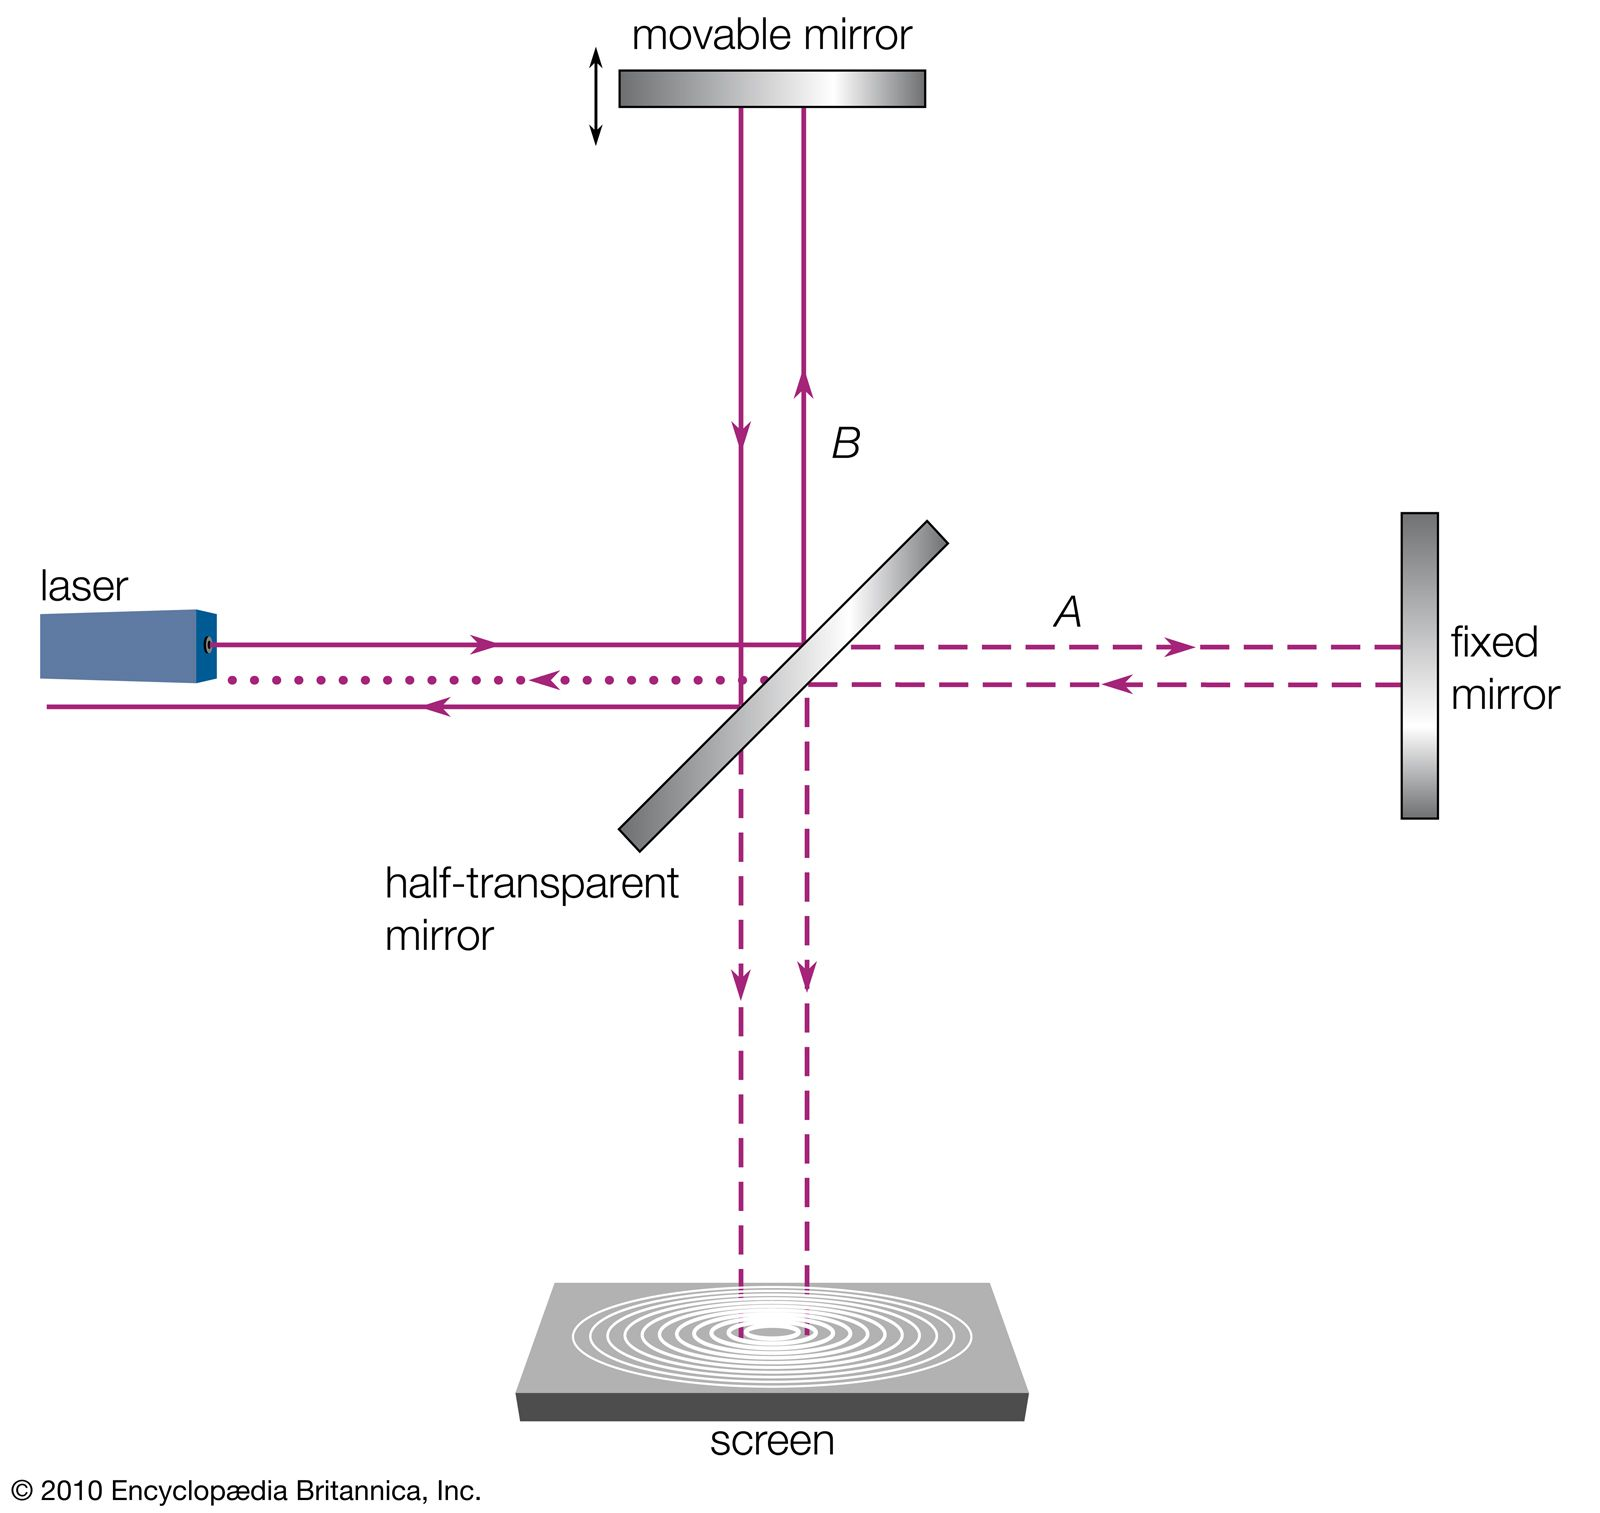
\includegraphics[width=0.8\textwidth]{images/michaelson_interferometer.jpg}
    \end{center}
    \caption{Schematic representation of a Michelson interferometer. A laser beam is split by a half-transparent mirror into two orthogonal arms of length $L_A$ and $L_B$.
    The beams reflected from the mirrors are recombined at the detector (screen), where, if a gravitational wave has passed, they produce an interference pattern.
    Variations in the optical path length of one arm (through the movable mirror) shift the observed fringes.
    The source for this image is at \url{https://www.britannica.com/technology/Michelson-interferometer}.}
    \label{fig: michaelson interferometer}
\end{figure}
The laser is used to have a monochromatic light source, with a frequency $\omega_L$, a wave-vector $k_L=\omega_L/c$ and a wavelength $\lambda_L = 2\pi/k_L$.
Therefore, referring to \textbf{Figure~\ref{fig: michaelson interferometer}}, we label as A and B respectively the $x$ and $y$ arms of the interferometer, with lengths $L_A$ and $L_B$.
If $t_0$ is the time the beam reaches the beam splitter the first time, it will come back to it from the two paths at time $t = t_0 + 2L_{A}/c$ and $t'= t_0 + 2L_B/c$.
The detector only sees one single recombined beam, not two beams arriving at different times, so in its perspective, if one had to cross a longer distance than the other it had to have started its journey before the other, meaning $t\equiv t'$, and the two beams start at $t_0^{(A)} = t - 2L_A/c$ and $t_0^{(B)} = t - 2L_B/c$.
If we set the beam splitter at the origin of the frame, this initial time difference translates in a phase difference between the two separate beans. 
If the phase is conserved during the free propagation, there are some factors acquired by the field during the reflections and refractions, and the overall effect gives the two electric fields that will recombine at the beam splitter as
\begin{equation}
    \left\{
        \begin{aligned}
            &E_1 = -\frac{1}{2}E_0e^{-i\omega_Lt + 2ik_LL_A} \\
            &E_2 = -\frac{1}{2}E_0e^{-i\omega_Lt + 2ik_LL_A},
        \end{aligned}
    \right.
    \label{eq: fields in arms of michaelson}
\end{equation}
The total electric field is the sum of the two, and after some re-writing it can be shown that the power measured by the photodetector is 
\begin{equation}
    |E_{out}|^2 = E_0^2 \sin^2[k_L(L_A-L_B)],
    \label{eq: power measured by photodetector}
\end{equation}
therefore any variation in the lengths of the two arms corresponds to a variation in the power measured at the photodetector.
Note that, since $k_L=2\pi/\lambda_L$, the~\eqref{eq: power measured by photodetector} becomes
\begin{equation*}
    |E_{out}|^2 = \frac{1}{2} E_0^2 \left[1-\cos{\left(\frac{4\pi}{\lambda_L}\Delta L\right)}\right],
\end{equation*}
therefore the detector measures a value depending on the cosine, which in turn depends on $\Delta L$: if there is no gravitational wave, I would expect a null measure.

\subsubsection{Gravitational waves and TT gauge}
The TT gauge describes the position of \textit{free falling} objects, that does not change when a gravitational wave passes. 
In order to replicate this condition the mirrors of the interferometers should also be "free falling", but instead their fall is halted by suspensions.
This apparent problem is solved when considering that the effects of gravitational waves are perpendicular to their direction of motion, and therefore the mirrors need to be decoupled in the horizontal plane, rather than the vertical.
For this reason, the mirrors are suspended, and as far as the motion in the horizontal plane is concerned they can be taken to be following the geodesics of the time-dependent part of the gravitational field.
Thus, in the TT gauge the coordinates of the beam splitter (at the origin) and of the mirrors - at $(L_A,0)$ and $(0,L_B)$ - are not affected by the passage of a wave, but the propagation of light in the arms is.
Assuming a \textit{plus-polarized} gravitational wave moving in the $z$ direction, perpendicular to the plane defined by the two arms, we have 
\[
    h_+(t)=h_0\cos{\omega_{gw}t},
\]
and the space-time interval in the TT frame will be given by
\[
    ds^2= -c^2dt^2 + [1+h_+ (t)]dx^2 + [1- h_+(t)]dy^2 + dz^2.
\]
Since photons follow the null geodesic, we can set $ds=0$, and, considering the arm in the x direction as an example, we get 
\[
    dx = \pm cdt\left[1-\frac{1}{2}h_+(t)\right], 
\]
where the sign depends on the direction of motion with respect to the origin. 
These can be used to write the length of the arms as the time integral from the beam splitter at $t_0$, to the mirror at time $t_1$, or from this time back to the beam splitter, at $t_2$, in order to find the total time interval in which the light has traveled along the arms.
By neglecting terms $O(h^2)$, and using some trigonometric identities, we can find the time interval for the $x$-axis arm as 
\begin{equation}
    t_2-t_0 = \frac{2L_A}{c} + \frac{L_A}{c}h(t_0+L_A/c)\frac{\sin{(\omega_{gw}L_A/c)}}{(\omega_{gw}L_A/c)},
    \label{eq: time interval for x-axis}
\end{equation}
where 
\[
    sinc\hspace{1mm}\left(\frac{\omega_{gw}L}{c}\right) \equiv \frac{\sin{(\omega_{gw}L_A/c)}}{(\omega_{gw}L_A/c)}\xrightarrow{\frac{\omega_{gw}L}{c}\to0}1.
\]
Therefore, when the period of the gravitational wave is large with respect to the time it takes the light to travel along the arm, the $\Delta t$ shift in the travel time $t_2 - t_0$, with respect to the unperturbed case is simply $h(t_1)L_A/c$.
In the opposite case, when $\omega_{gw}L_A/c \gg 1$, $h(t)$ will change sign many times during the travel time, making its net contribute $\sim0$.
Now, from~\eqref{eq: time interval for x-axis} and its $y$-axis counterpart, it is possible to find the two different starting time we have talked about, $t_0^{(x)}$ and $t_0^{(y)}$\footnote{Note that if $L_A=L_B=L$, and $\frac{\omega L}{c}\ll 1$, the difference between the two would be
\[
    t_0^{(y)} - t_0^{(x)} = \frac{2L}{c} h\left(t-\frac{L}{c}\right)sinc\hspace{1mm}(\omega L/c)\approx \frac{2L}{c}h\left(t-\frac{L}{c}\right).
\]
}. 
By substituting them in the electric field expressions in~\eqref{eq: fields in arms of michaelson} we can find
\begin{equation}
    \left\{
        \begin{aligned}
            E^{(x/y)} &= \mp\frac{1}{2}E_0e^{-i\omega_L t_0^{(x/y)}} \\
            \vspace{1mm}
                      &= \mp\frac{1}{2}E_0e^{-i\omega_L \left(t-\frac{L_{A/B}}{c}\right)+i\Delta\phi_{x/y}(t)},
        \end{aligned}
    \right.
    \label{eq: field in interferometer}
\end{equation}
where
\begin{equation}
    \Delta\phi_{x/y}= \pm h_0 \frac{\omega_L L_{A/B}}{c} sinc\hspace{1mm}(\omega_{gw}\frac{L_{A/B}}{c})\cos{\left[ \omega_{gw}(t - \frac{L_{A/B}}{c}) \right]},
    \label{eq: field phase interferometer}
\end{equation}
is the phase difference from the unperturbed case in the two arms.
Generally, $L_A$ and $L_B$ are made to be as similar as possible, therefore we can replace them with $L=(L_A - L_B)/2$ in~\eqref{eq: field phase interferometer}. 
We still consider the minimal differences between the two in~\eqref{eq: field in interferometer}, which can be rewritten\footnote{By using $2L_{A/B} = 2L \pm (L_A - L_B)$.} as 
\begin{equation*}
    E^{(x/y)}(t) = \mp \frac{1}{2}E_0 e^{-i\omega_L(t-2L/c) \pm i\phi_0 + i\Delta\phi_{x/y}(t)},
    \notag
\end{equation*}
where
\begin{equation}
    \phi_0 = k_L(L_A - L_B),
    \label{eq: programmable phase difference}
\end{equation}
is a phase parameter that the experimenter can adjust.
The strategy to build a "null instrument", which records zero signal when the gravitational wave is not passing, by setting $L_A = L_B \to \phi_0=0$, turns out to be failing, since it makes the instrument insensitive to calibration uncertainties.
At the same time, setting the instrument to a phase where the variation is maximum, as for $\phi_0=\pi/4$, makes the instrument too sensible, so much that it will not be able to distinguish a signal from the laser power fluctuations.
Therefore, depending on how this parameter is adjusted the instrument can be more or less sensible to signal variations, and the best value tends to be between these two extremes.

\subsection{LISA}
Ground-based detectors such as LIGO and Virgo have pioneered the technique we have just shown in the high-frequency band ($\gtrsim 10$~Hz).
The purpose for future space-based interferometers like LISA is to extend it to the low-frequency regime, opening a new observational window on astrophysical and cosmological sources.
Indeed, space-based detectors such as LISA will be sensitive to DWDs with periods of a few hours down to a few minutes.  
At the shortest periods, these binaries are in very tight orbits, with separations of only a few $10^{4}$–$10^{5}$~km, comparable to Earth's diameter.
Between the binary systems, the interacting ones can have extremely short orbital periods ($\lesssim 10$ minutes) and are strong, nearly monochromatic gravitational wave sources over LISA's lifetime.  
Detached systems with periods in the mHz range are also important, as they provide long-lived, stable signals that can serve as calibration sources or ``verification binaries'' for space-based detectors.
Given their abundance and gravitational wave luminosity, binary white dwarfs are expected to be the most numerous class of resolvable sources for LISA, and their unresolved population will form a significant component of the low-frequency gravitational wave foreground.

\subsubsection{Instrument description}
Earth-based detectors are limited in sensitivity in the low frequencies by sysmic noise, gravity gradients from local mass movements, etc.
Basing new detectors allows to eliminate these sources of noise, allowing to explore a frequency regime which contains precious information ob many interesting astrophysical sources, such as DWDs, extreme mass-ratio inspirals and massive black hole mergers.
In LISA's case, the arms are not going to be physical structures, but $2.5\times10^6$km separations between three identical spacecrafts at the vertices of an equilateral triangle.
Each one of the spacecraft will host two free-falling test masses, isolated from all non-gravitational interactions by a drag-free control system.
The spacecrafts will trail by about $20^{\circ}$, with the triangular constellation inclined by $60^{\circ}$ to the ecliptic plane, following the earth around the sun.
With this configuration, it is possible to keep the long baseline stable, while having continuous source visibility, and a good localization (granted by the triangular shape).

\subsubsection{Frequency}
LISA's frequency band roughly covers the low range $0.1~\mathrm{mHz} \lesssim f \lesssim 1~\mathrm{Hz}$ (compared to LIGO's frequency of 10 Hz to 1000 Hz), corresponding to objects in much wider orbits and potentially much heavier than those that LIGO is searching for, opening up the detection realm to a wider range of gravitational wave sources. 
In this frequency range also reside most DWDs.  
In the low frequencies, the range is limited by the acceleration noise on the test masses: even in space, the "free" test masses are not completely isolated, but could be influenced by solar radiation and winds, and the "drag-free" micro-propellers that compensate these disturbances make noise under the $0.1mHz$. 
Also, in order to detect a very slow waves, LISA needs to observe it for at least one complete cycle, and if the wave has a period of months, the signal could become indistinguishable from a slow relative position change between the three satellites.
At the high frequencies, the main limits are due to the arms length, which make LISA unable to detect waves much shorter than that scale, and the power limits of the laser, which makes the photon count Poissonian noise more relevant at high frequencies.  
LISA’s sensitivity curve combines instrumental noise and the astrophysical foreground, including Galactic background and Galactic binary systems, as shown in \textbf{Figure~\ref{fig: LISA sens curve with noises}}. 
\begin{figure}
    \begin{center}
        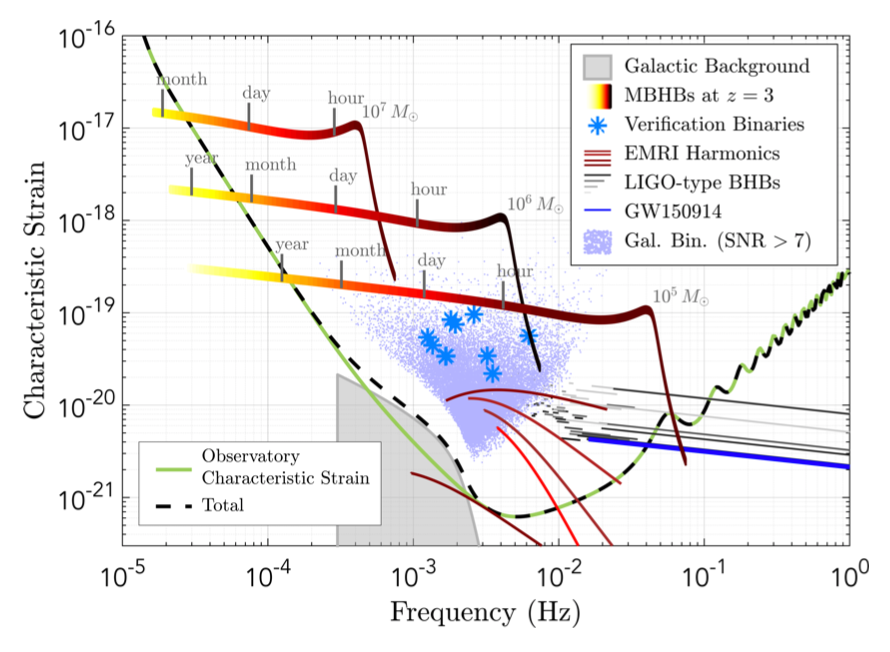
\includegraphics[width=0.7\textwidth]{images/lisa_sensitivity_with_noises.png}
    \end{center}
    \caption{LISA sensitivity curve in the characteristic strain representation.
    The solid green line shows the instrumental noise curve, while the dashed black line represents the LISA curve as shaped by the background contribution from unresolved Galactic binaries.
    Different astrophysical sources that emit gravitational wave signal in this band are indicated: massive black hole binaries (MBHBs), extreme mass-ratio inspiral (EMRI), stellar-mass black hole binaries, verification binaries, and Galactic binaries with signal-to-noise ratio larger than 7.
    The source for this image is~\url{https://ar5iv.labs.arxiv.org/html/1803.01944}}\label{fig: LISA sens curve with noises}
\end{figure}
As far as the frequency resolution of a coherent observation is concerned, the limits are not due to hardware, but the actual total observational time: in a Fourier analysis, this is set by the inverse of the total observation time:  
\begin{equation}
\Delta f \approx \frac{1}{T_{\mathrm{obs}}}.
\end{equation}
For a nominal mission duration of $T_{\mathrm{obs}} \simeq 4$~years, $\Delta f \approx 8\times 10^{-9}$~Hz, allowing very fine separation of closely spaced monochromatic sources.

\subsubsection{Why white dwarfs}
As shown in \textbf{Figure~\ref{fig: LISA sens curve with noises}}, we expect the Galactic binaries to generate a confusion foreground that is able to shape the LISA sensitivity curve, mostly due to their proximity and large number.
The purpose of this work, however, is to discover if the extra-galactic binaries, despite their much grater distance, are sufficiently numerous to generate an overall detectable stochastic gravitational wave background in the LISA band.
In particular, from a scientific perspective, DWDs offer a rich laboratory:  
\begin{itemize}
    \item The DWDs binary systems typically are in compact orbits, and the corresponding frequencies easily fall in LISA's band; 
    \item The DWDs are some of the most common compact systems in the universe, that represent a probable output for binary system evolutions. 
    When the number of non-resolvable sources is big, their signals superpose stochastically, generating a background; 
    \item We have found a simple and predictable shape for their signal, in~\eqref{eq: the strain we use}, which is easy to simulate, and allows to generate coherent synthetic populations with astrophysical models; 
    \item As we said, we already expect galactic binaries to affect LISA's curve, therefore it is a natural realistic candidate to test;
\end{itemize}
The combination of abundance, signal strength, and astrophysical relevance makes them a target for LISA’s mission that is worth exploring further.

